\documentclass[10pt]{article}
\usepackage{graphicx}
\usepackage[margin=1.5cm]{geometry}
\usepackage{amsmath}
\def\brcurs{{\mbox{$\resizebox{.16in}{.08in}{
\includegraphics{BoldR}}$}}}
\def\brcurs{{\mbox{$\resizebox{.16in}{.08in}{
\includegraphics{ScriptR}}$}}}

\begin{document}
\twocolumn

\title{Thursday Warm-up: Vector Algebra and Calculus Review}
\author{Prof. Jordan C. Hanson}

\maketitle

\section{Memory Bank}

\begin{itemize}
\item Spherical coordinates:
\begin{enumerate}
\item $x=r\sin\theta\cos\phi$, $y=r\sin\theta\sin\phi$, $z=r\cos\theta$.
\item $\mathbf{A} = A_r\hat{\mathbf{r}} + A_\theta\hat{\boldsymbol{\theta}} + A_\phi\hat{\boldsymbol{\phi}}$
\item $\hat{\mathbf{r}}=\sin\theta\cos\phi\hat{\mathbf{x}}+\sin\theta\sin\phi\hat{\mathbf{y}}+\cos\theta\hat{\mathbf{z}}$
\item $\hat{\boldsymbol{\theta}}=\cos\theta\cos\phi\hat{\mathbf{x}}+\cos\theta\sin\phi\hat{\mathbf{y}}-\sin\theta\hat{\mathbf{z}}$
\item $\hat{\boldsymbol{\phi}}=-\sin\phi\hat{\mathbf{x}}+\cos\phi\hat{\mathbf{y}}$
\item $d\mathbf{l}=dr\hat{\mathbf{r}}+rd\theta\hat{\boldsymbol{\theta}}+r\sin\theta d\phi\hat{\boldsymbol{\phi}}$
\item $d\tau = r^2\sin\theta dr d\theta d\phi$
\item $\nabla T = \left(\frac{\partial T}{\partial r}\right)\hat{\mathbf{r}} + \left(\frac{1}{r}\frac{\partial T}{\partial \theta}\right)\hat{\boldsymbol{\theta}} + \left(\frac{1}{r\sin\theta}\frac{\partial T}{\partial \phi}\right)\hat{\boldsymbol{\phi}}$
\item 
\begin{multline}
\nabla \cdot \mathbf{v}=
\frac{1}{r^{2}} \frac{\partial}{\partial r}\left(r^{2} v_{r}\right)+
\frac{1}{r \sin\theta} \frac{\partial}{\partial \theta}\left(\sin\theta v_{\theta}\right)+\\
\frac{1}{r \sin\theta} \frac{\partial v_{\phi}}{\partial \phi}
\end{multline}
\item 
\begin{multline}
\nabla \times \vec{v}= \\ \left[\frac{1}{r \sin\theta} \left( \frac{\partial}{\partial \theta} \left( \sin\theta v_{\phi} \right)-\frac{\partial v_{\theta}}{\partial \phi} \right)\right] \hat{\mathbf{r}}+ \\ 
\left[\frac{1}{r}\left( \frac{1}{\sin\theta} \frac{\partial v_{r}}{\partial \phi}-\frac{\partial}{\partial r}\left( r v_{\phi}\right)\right)\right]\hat{\boldsymbol{\theta}}+ \\ 
\left[\frac{1}{r} \left( \frac{\partial}{\partial r}\left( r v_{\theta} \right)-\frac{\partial v_{r}}{\partial \theta} \right)\right] \hat{\boldsymbol{\phi}}
\end{multline}
\end{enumerate}
\end{itemize}

\begin{figure}[hb]
\centering
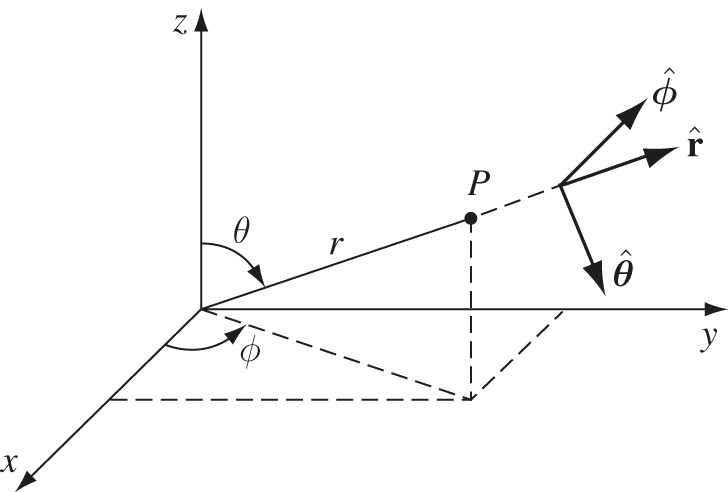
\includegraphics[width=0.28\textwidth]{figures/1_36.jpg}
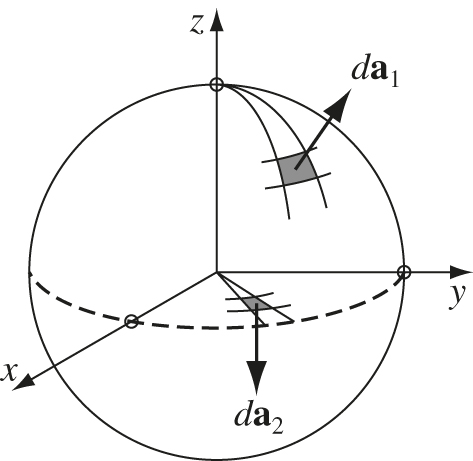
\includegraphics[width=0.2\textwidth]{figures/1_39.jpg}
\caption{\label{fig:1} Spherical coordinate system.}
\end{figure}

\section{Review: Vector Calculus with \\ Spherical Coordinates}

\begin{enumerate}
\item (a) Suppose the radius of the Earth is 6371 km.  What is the circumference of the Artic circle, at a latitude of 65.825 degrees North? (b) Prove that the volume of a sphere is $(4/3) \pi R^3$, and calculate the volume of the Earth. (c) Assume a reasonable value for the average density of Earth, and calculate the mass of our planet. (d) Which unit vector in spherical coordinates corresponds to changes in longitude?  Latitude?  What are the equivalent Cartesian unit vectors at the equator, and the \textit{prime meridian} (where longitude is zero)? \\ \vspace{4cm}
\item (a) What is the gradient of $f(r) = k/r$? (b) What is the divergence of $\mathbf{v} = \hat{\mathbf{r}}/r^2$? (c) Check the divergence theorem using $\mathbf{v}$ and the unit sphere as the surface. \\ \vspace{3cm}
\item Let $\mathbf{v} = (1/r^2)\hat{\mathbf{r}}+k\hat{\boldsymbol{\phi}}$. Evaluate the following integral over the unit circle in the xy-plane\footnote{\textit{What fundamental theorem tool do you have to solve this?}}.
\begin{equation}
I = \int_{S} (\nabla \times \mathbf{v}) \cdot d\mathbf{a}
\end{equation}
\end{enumerate}

\end{document}
